\chapter{Orchestration using Heat}
\gls{Heat} is the name of the OpenStack orchestration engine, which
can manage complete configurations of all servers, volumes, users,
networks and routers that make up a cloud application.  Instead of
managing every component separately, we can create, start, stop or
clean up our complete application in a single step.  Such a set of
collectively managed resources is called a \gls{stack}.

\gls{Heat} has its own dashboard interface, which you can find under
the Orchestration tab of the main OpenStack dashboard.  Official
documentation for Heat and its dashboard interface can be found at the
following locations:
\begin{itemize}
\item \url{https://docs.openstack.org/heat}
\item \url{https://docs.openstack.org/heat-dashboard}
\end{itemize}

\section{\gls{Heat Orchestration Template}s}
A \gls{stack}'s resources and their mutual dependencies can be
specified in a text file, called a \gls{Heat Orchestration Template}
(\textsc{HOT}).  The syntax of these templates conforms to the
\gls{YAML} standard, for which many text editors provide specialized
editing modes.  The following example describes a stack consisting of
a single VM:
\begin{code}{}
heat_template_version: 2018-03-02

description: Deploy a single compute instance

parameters:
  user_network:
    type: string
    label: user_network
    description: Add the required VM network
    constraints: [ custom_constraint: neutron.network ]
  user_key:
    type: string
    label: ssh_user_key
    description: Public ssh key for user authentication
    constraints: [ custom_constraint: nova.keypair ]

resources:
  my_instance:
    type: OS::Nova::Server
    properties:
      security_groups: [ default ]
      networks: [ network: { get_param: user_network } ]
      key_name: { get_param: user_key }
      image: Ubuntu_16.04_2NICs
      flavor: m1.small
\end{code}

Our example contains four main sections:
\begin{description}
\item[\texttt{heat\_template\_version}] The \textsc{HOT} specification
  has evolved since its initial release.  The key
  \lstinline{heat_template_version} indicates the version of the
  syntax used in this template.  It's value can be a release date or
  (in recent version) the name of the version.
\item[\texttt{description}] A description is optional, but
  recommended.
\item[\texttt{parameters}] An optional section, \lstinline{parameters}
  allow users to configure various properties when instantiating a new
  stack, without having to edit the template itself.  A parameter
  value can be used elsewhere in the template using the function
  \lstinline{get_param}.
\item[\texttt{resources}] This section contains all the resources used
  by the Stack.  In this case, there is just a single VM instance.
\end{description}
Optional additional sections are \lstinline{parameter_groups},
\lstinline{outputs}, and \lstinline{conditions}.

The official OpenStack template documentation at
\url{https://docs.openstack.org/heat/latest/template_guide} contains a
specification of the \textsc{HOT} format, as well as information on
how to describe the various types of resources in a template.
\textsc{VSC} also provides some example templates in the repository
\url{https://github.com/hpcugent/openstack-templates}.

\section{The Template Generator}\label{sec:template-generator}
The Heat dashboard provides a graphical interface where users can draw
templates by dragging resources onto a canvas, and connecting them.
Users can then download a template generated from this interface, or
immediately instantiate it as a stack.

As an example, we will create a template for a single node attached to
a floating IP from the public pool, making it accessible from outside
the OpenStack cloud.  It might be useful to compare this approach to
that of the example in the official documentation at
\url{https://docs.openstack.org/heat/latest/template_guide/basic_resources.html#os-neutron-resources}.

\begin{enumerate}
\item Open the Template Generator from the Orchestration tab.  Here,
  you are presented with a set of icons for the different resources,
  and a canvas.  The floppy disk icon (``Manage Drafts'') allows you
  to save and restore different versions of your work.
  \begin{center}
    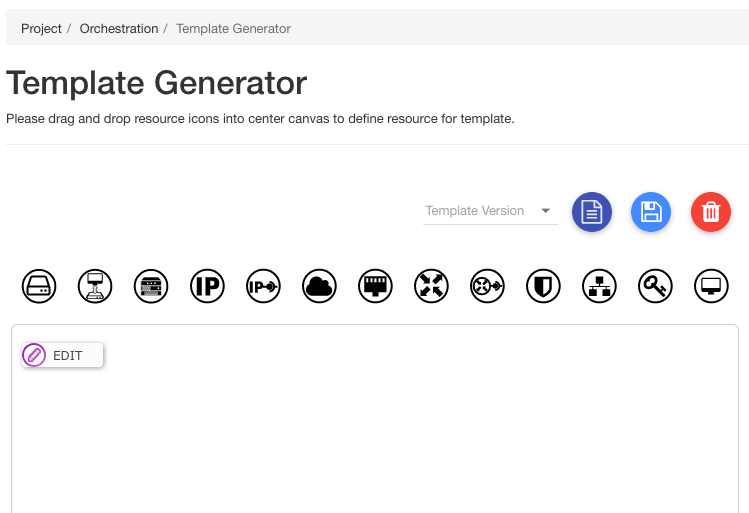
\includegraphics[width=0.7\textwidth]{img/template_generator}
  \end{center}
\item You can now drag and drop icons onto the canvas to add resources
  to the template.  Add a VM (OS::Nova::Server), a port
  (OS::Neutron::Port), a floating ip (OS::Neutron::FloatingIP), and a
  floating ip association (OS::Neutron::FloatingIPAssociation).
  \begin{center}
    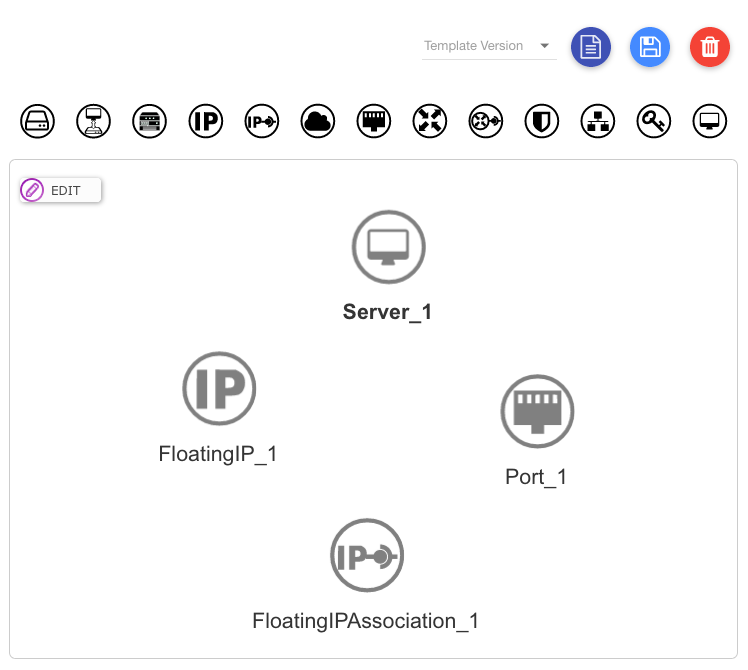
\includegraphics[width=0.7\textwidth]{img/all_resources}
  \end{center}
\item To associate the port to the server, draw a connection between
  Server\_1 and Port\_1.  To do this, click the purple ``EDIT'' icon,
  select ``ADD EDGE'', and click and drag to draw an edge from
  Server\_1 to Port\_1.  This will make Port\_1 a port of Server\_1.
  Note that edges are directed: you can't draw an edge from Port\_1 to
  Server\_1.  The resource at the end-point of an edge becomes a
  property of the resource at the starting point.
  \begin{center}
    \includegraphics[width=0.7\textwidth]{img/draw_edge}
  \end{center}
\item In the same way, draw an edge from FloatingIPAssociation\_1 to
  Port\_1, and from FloatingIPAssociation\_1 to FloatingIP\_1.  The
  stack's graph should now look as follows:
  \begin{center}
    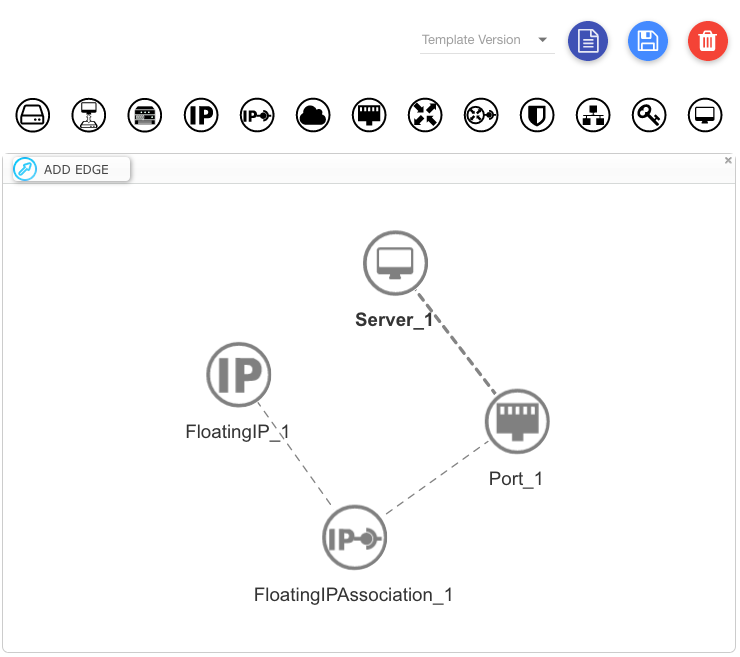
\includegraphics[width=0.7\textwidth]{img/all_resources_connected}
  \end{center}
\item Next, specify the required properties of each resource.
  Left-clicking a resource opens up a window with properties.
  \begin{itemize}
  \item For Server\_1, configure a VM flavor and boot source in the
    ``BASIC'' tab.  In the ``ACCESS \& SECURITY'' tab, select a public
    key for authentication.  You can also have a look at the
    ``Networks'' tab, where you should see that a ``port'' property
    for Port\_1 has been added automatically.  Click ``SAVE'' to save
    your settings and close the property window.
    \begin{center}
      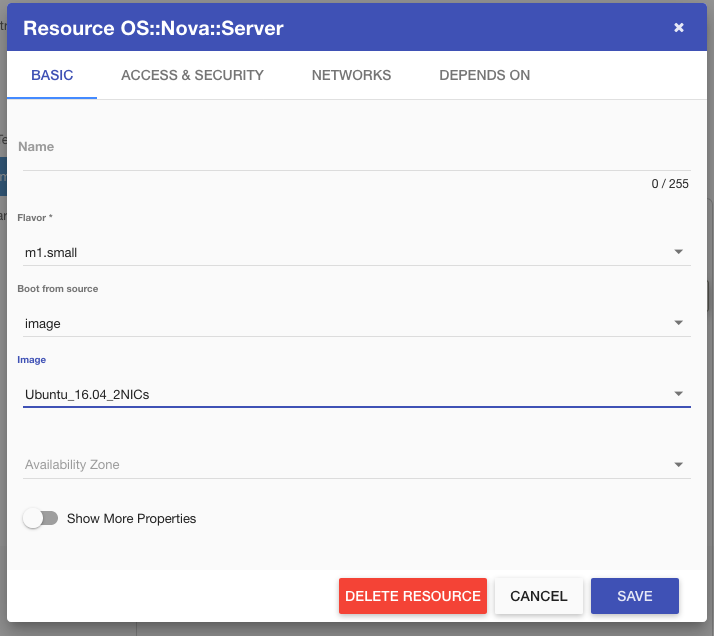
\includegraphics[width=0.7\textwidth]{img/server_basic_properties}
      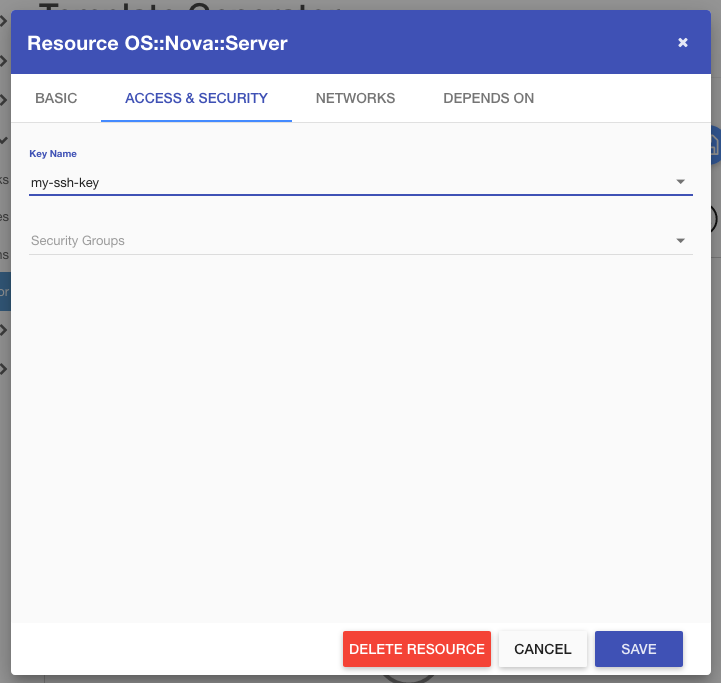
\includegraphics[width=0.7\textwidth]{img/server_access_security}
      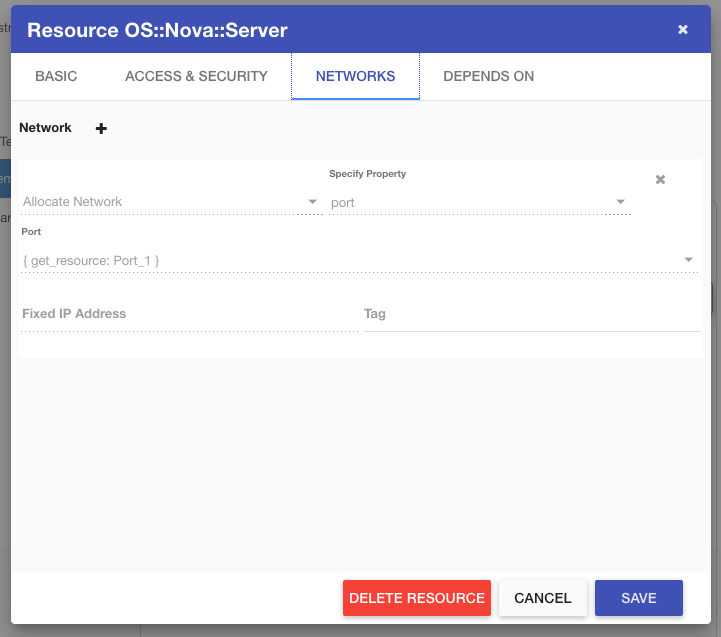
\includegraphics[width=0.7\textwidth]{img/server_networks}
    \end{center}
  \item In the properties for Port\_1, you should select the ``vm''
    network in ``Network'', enable at least the ``default'' security
    group, and check ``Port Security Enabled''.  Click ``SAVE''.
    \begin{center}
      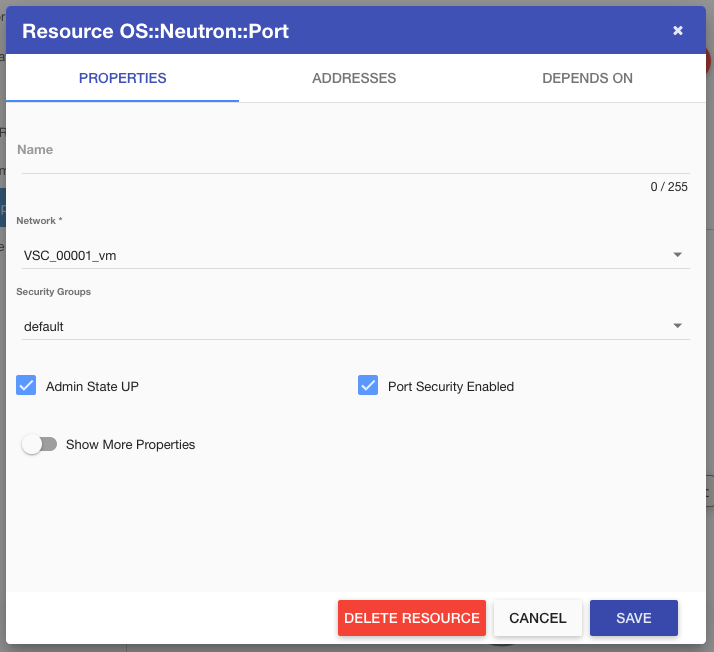
\includegraphics[width=0.7\textwidth]{img/port_properties}
    \end{center}
  \item Choose the network for FloatingIP\_1.  Select the ``public''
    network to obtain a public floating ip, which will allow outside
    access to your VM.  Click ``SAVE''.
    \begin{center}
      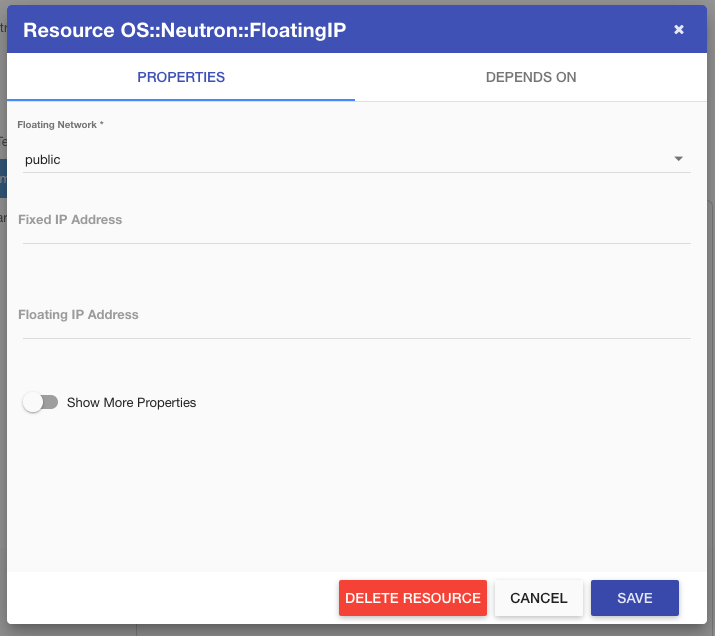
\includegraphics[width=0.7\textwidth]{img/floatingip_properties}
    \end{center}
  \item When you open up the properties window for
    FloatingIPAssociation\_1, you can see that the Floating IP and
    Port ID properties are set correctly.  However, you still need to
    click ``SAVE'' in order to be able to generate a template later
    on.
    \begin{center}
      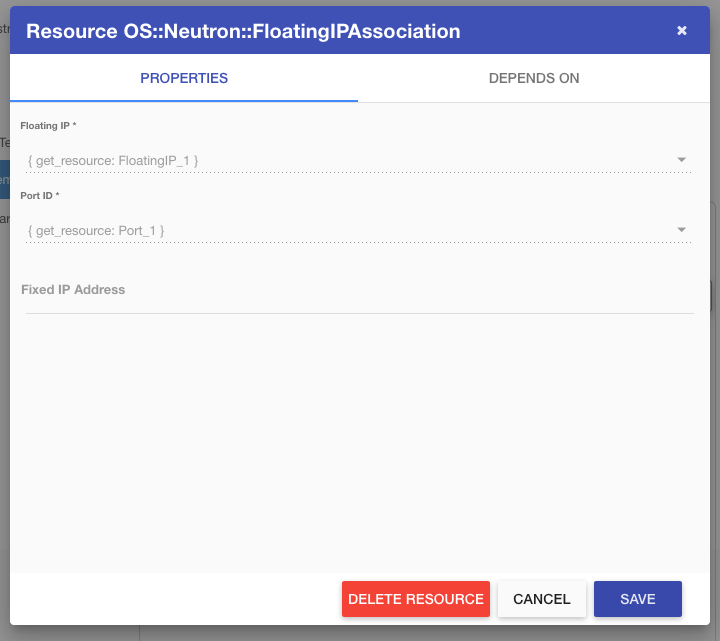
\includegraphics[width=0.7\textwidth]{img/floatingipassociation_properties}
    \end{center}
  \end{itemize}
\item When all required properties have been set and saved, all of the
  template's resources are drawn in a blue color.  We are now ready to
  generate a template from our configuration.
  \begin{center}
    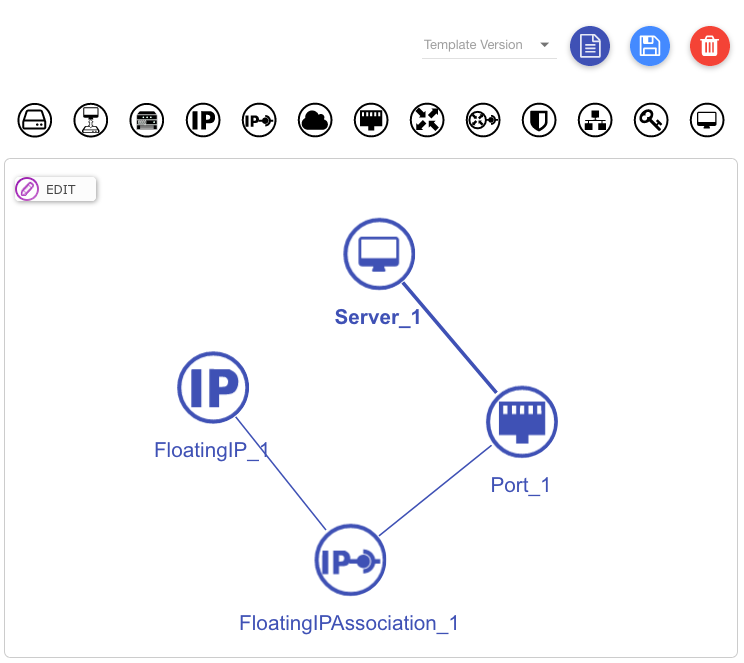
\includegraphics[width=0.7\textwidth]{img/stack_complete}
  \end{center}
\item In the ``Template Version'' drop-down menu, select the version
  of the HOT syntax you wish to use, e.g.\
  heat\_template\_version.2018-03-02.  Now you can click the document
  icon to see the generated template, which you can download, or
  immediately instantiate using ``CREATE STACK''.  \strong{Note:} clicking
  ``CREATE STACK'' takes you out of the template generator, with no
  option to resume working on the configuration, unless you save a
  draft first.
  \begin{center}
    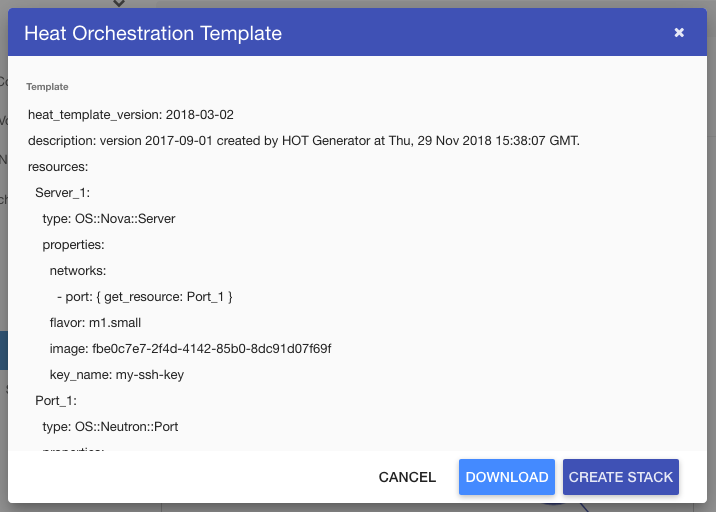
\includegraphics[width=0.7\textwidth]{img/complete_template}
  \end{center}
\end{enumerate}

The resulting template should look as follows:

\begin{code}{}
heat_template_version: 2018-03-02
description: version 2017-09-01 created by HOT Generator at Wed, 28 Nov 2018 13:45:30 GMT.
resources:
  FloatingIP_1:
    type: OS::Neutron::FloatingIP
    properties:
      floating_network: fc06776a-02df-4962-8513-aea8b8177fd2
  FloatingIPAssociation_1:
    type: OS::Neutron::FloatingIPAssociation
    properties:
      floatingip_id: { get_resource: FloatingIP_1 }
      port_id: { get_resource: Port_1 }
  Port_1:
    type: OS::Neutron::Port
    properties:
      admin_state_up: true
      security_groups:
        - 462946d4-aec5-400c-848b-edd916760b25
      network: 2a6d5e54-91b9-4e47-8692-409f4ce1e1c8
      port_security_enabled: true
  Server_1:
    type: OS::Nova::Server
    properties:
      networks:
        - port: { get_resource: Port_1 }
      flavor: m1.small
      image: fbe0c7e7-2f4d-4142-85b0-8dc91d07f69f
      key_name: my-ssh-key
\end{code}

Not all features of OpenStack templates, such as template parameters,
are available in the template generator, but a generated template can
serve as a starting point for more advanced configurations.

\section{Launching a stack}

%%% Local Variables:
%%% mode: latex
%%% TeX-master: "intro-OpenStack"
%%% End:
